\chapter{User Interface Design and Implementation}

\section{Updated pages}
A few changes were brought in addition to our original designs, which are highlighted in this section.
\subsection{Finalized Header}
To bring a consistant theme to the whole website, a header is there to help. We had a header in the last version of the report but we needed navigable tabs to get around the website that will appear on every page, as well as a search bar for quick access to something more specific. Referring to the figure below, one can see that the new header removed the need to have a sidebar and therefore saves space and makes the end result more pleasing to the user. 
\begin{figure}[H]
\centering

\includegraphics[width=5.5in]{./mockups/JPEG/headernew.jpg}
\caption{The header located on the top of every page.}
\end{figure}

\subsection{Finalized League page}
The last league page was a bit cluttered with the top three users section, and therefore a change was needed. This change brings about a cleaner representation of the top three users in a league and also an easier design to implement in the end. Bootstrap comes equipped with an accordian widget which has a main section that highlights content and a few buttons that change the content that is being shown, all while providing a clean animation on top of that. We will take advantage of that widget because it looks great and is easy to make.
\begin{figure}[H]
\centering
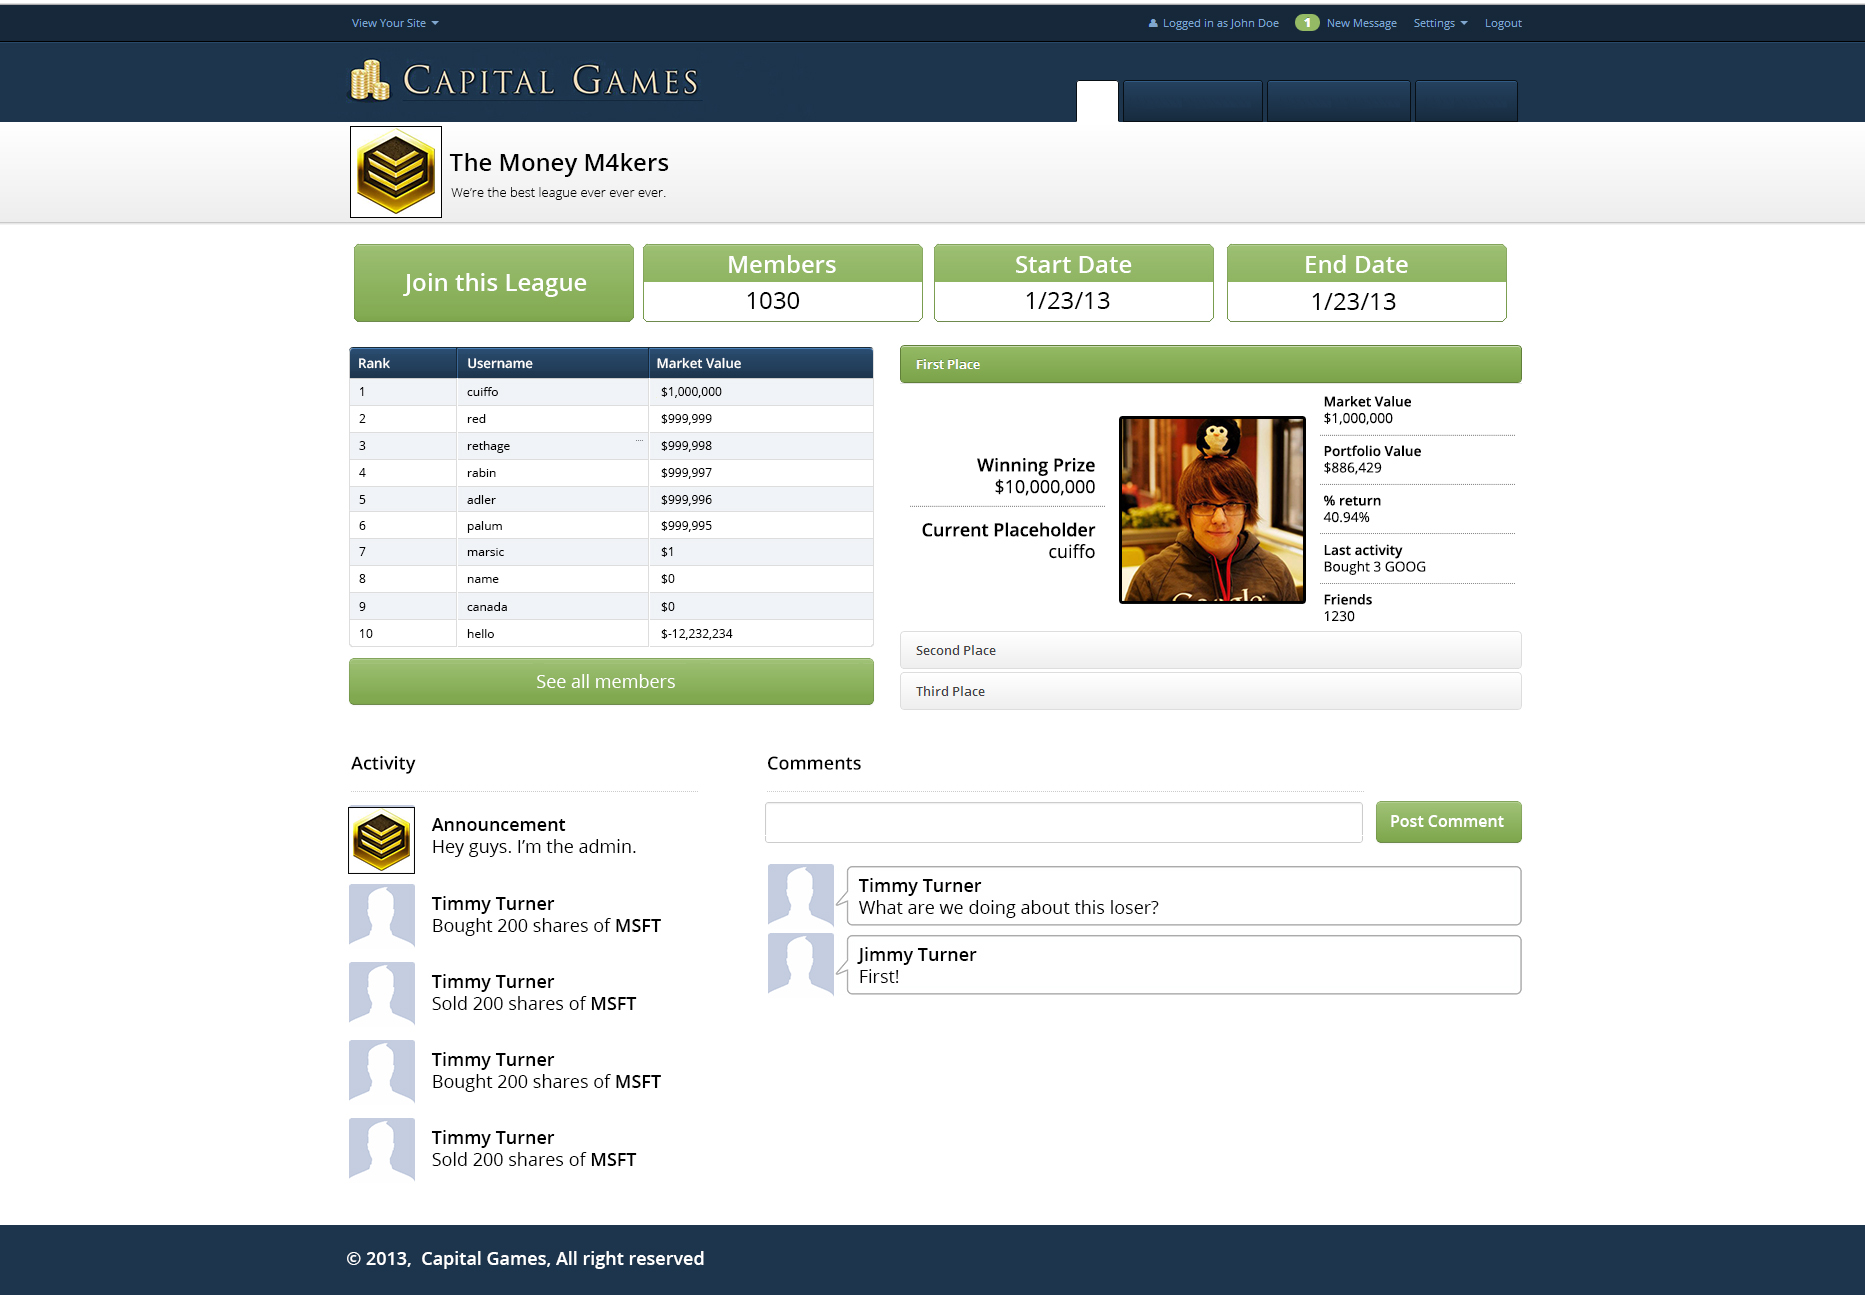
\includegraphics[width=5.5in]{./mockups/JPEG/Leaguesfourth.jpg}
\caption{Changes to the leagues page.}
\end{figure}

\subsection{Initial Front Page}
The initial designs also lacked a page that a user is brought to when they first visit out website. A user cannot simply be taken to a login/sign up page without being told anything about the website or being greeted. This new page works as the page a visitor who is not logged in is brought to so they can choose the necessary action. For a user that already has an account, they can choose to log in via the leftmost button or the link up top. For a user that wants to create an account, they can choose to do so by clicking the middle button that will redirect to a simple form. For a user that wants to learn more about us, they can press the rightmost button which will bring them to the interactive tutorials we be implementing. 
\begin{figure}[H]
\centering

\includegraphics[width=5.5in]{./mockups/JPEG/initialpage.jpg}
\caption{The page a user who is not logged in sees when they first visit our website.}
\end{figure}


\section{Efficiency of the views}
Our website has to be efficient but also not be a terrible pain to the programmers. There are a few ways that this can be dealt with on the view-side of programming.
\subsection{Separation of the header and content}
Ruby on Rails provides a feature that facilitates the creation of pages by having one page that is always loaded and somewhere in the middle it is redirected to the actual content. This means, for us, that we can create the content for each page and then rather than have to make the header each time, we can create that once and then link the content in the header page. On each page load, the header will be loaded and then the code will have a link which will then go find the correct file that contains the content code. Two reasons why this method is great are the ease to the programmer and the fact that the data will be stored in cache because we are loading the same exact file on the second page, therefore making loading much more efficient.
\subsection{Avoiding long loading times}
There are several ways we can reduce the amount of time the end user is going to have to wait for the page to load. One easy thing to do is that any pictures that we include should be scaled down to whatever is the maximum size it will be at. Having a large image and downscaling it is a waste of resources. Also on that topic, whenever a user uploads a picture, we will scale those down to a 100x100 icon. Another way we can avoid long loading times is to rely less on images and create pages with all code unless absolutely necessary. This is just good programming practice because loading images when you can create something through code is a waste of bandwidth and loading time. 
\subsection{Cross compatibility}
We decided to use Bootstrap elements to create our site, which comes with many features that help the programmer by predefining some views that are good-looking and cross compatible with all modern browsers and some older browsers that are still in use. In the case that we make some more features to the site that require non-Bootstrap elements, we can use the tool ``Modernizr'', which detects any features we are using that will not be supported in older browsers and correct them so that they work there, too.\cite{wiki:modern} It is an invaluable tool that will keep our pages current and universal.

